\documentclass[11pt]{article}
\usepackage[utf8]{inputenc}
\usepackage[T1]{fontenc} % uses T1 fonts (better quality)
\usepackage{lmodern} % uses Latin Modern fonts
\usepackage[margin=1in]{geometry}
\usepackage[dvipsnames]{xcolor}
\usepackage{ragged2e}
\renewcommand{\baselinestretch}{1.15}
\usepackage{tikz}
\usetikzlibrary{automata,scopes,shapes,matrix,arrows,decorations.pathmorphing}
\tikzset{>={stealth}}
\usepackage{amsmath,amsfonts,amssymb}
\usepackage{bm}
\usepackage{graphicx}
\usepackage[makeroom]{cancel}
\definecolor{OuterBlue}{HTML}{1370AA}
\definecolor{InnerBlue}{HTML}{9BC4DD}
\usepackage{pdfpages}

\begin{document}
 	\begin{center}
 	\LARGE{ECE 345 / ME 380: Introduction to Control Systems\\Problem Set \#1}\\[1.5em]
 	\large David Kirby\\[1.5em]
 	\large \textbf{Due Thursday, September 3, 2020 at 3:30pm}\\[2.5em]
 	\end{center}

\begin{enumerate}
    \item (+5 points) Consider lateral control of a rocket with a gimbaled engine. The equations of motion describe the relationship between the pitch, \(\theta(t)\), the lateral deviation, \(h(t)\), and the torque, \(f(t)\), from the engine with constant rocket speed \(V\) and positive, constant values \(k_1,k_0\). Presume all initial conditions are zero.
    \begin{align}
        J\ddot{\theta}(t)&=-k_{1}\dot{\theta}(t)-k_{0}\theta(t)+f(t)\\
        \dot{h}(t)&=V\theta(t)\notag
    \end{align}
    \begin{enumerate}
        \item Find the transfer function representation for the system with input \(F(s)\) and output \(H(s)\).\\[1em]
        Transforms of equation (1)
        \begin{align*}
            Js^{2}\theta(s)&=-k_{1}s\theta(s)-k_{0}\theta(s)+F(s)\\
            sH(s)&=V\theta(s)
        \end{align*}
        From there, rearrange to obtain:
        \begin{align*}
            \frac{H(s)}{F(s)}&=\frac{V\cancel{\theta(s)}}{s\cancel{\theta(s)}\left(Js^{2}+k_{1}s+k_{0}\right)}\\
            &=\frac{V}{s\left(Js^{2}+k_{1}s+k_{0}\right)}
        \end{align*}
    \end{enumerate}
    \item (+10 points) Amplifiers often have a deadband region in which amplification has little effect.This may be modeled as a cubic equation \(y= 3x^3\), in which the input to the amplifier is \(x\), and the output, i.e., the amplified signal, is \(y\).
    \begin{enumerate}
        \item Create a linear approximation for the signal around \({x_0= 0.6}\).
        \begin{align*}
        y_0&=3{(0.6)}^3=0.648\\[0.5em]
        \frac{\partial y}{\partial x} |x_0 &= 9x_0^2=3.24\\[0.5em]
        \Delta y &= y-y_0=y-0.648\\[0.5em]
        \Delta x &= x-x_0=x-0.6\\
        y&= 3.24(x-0.6)+0.648\\&=3.24x-1.296
        \end{align*}\newpage
        \begin{figure}[h!]
            \centering
            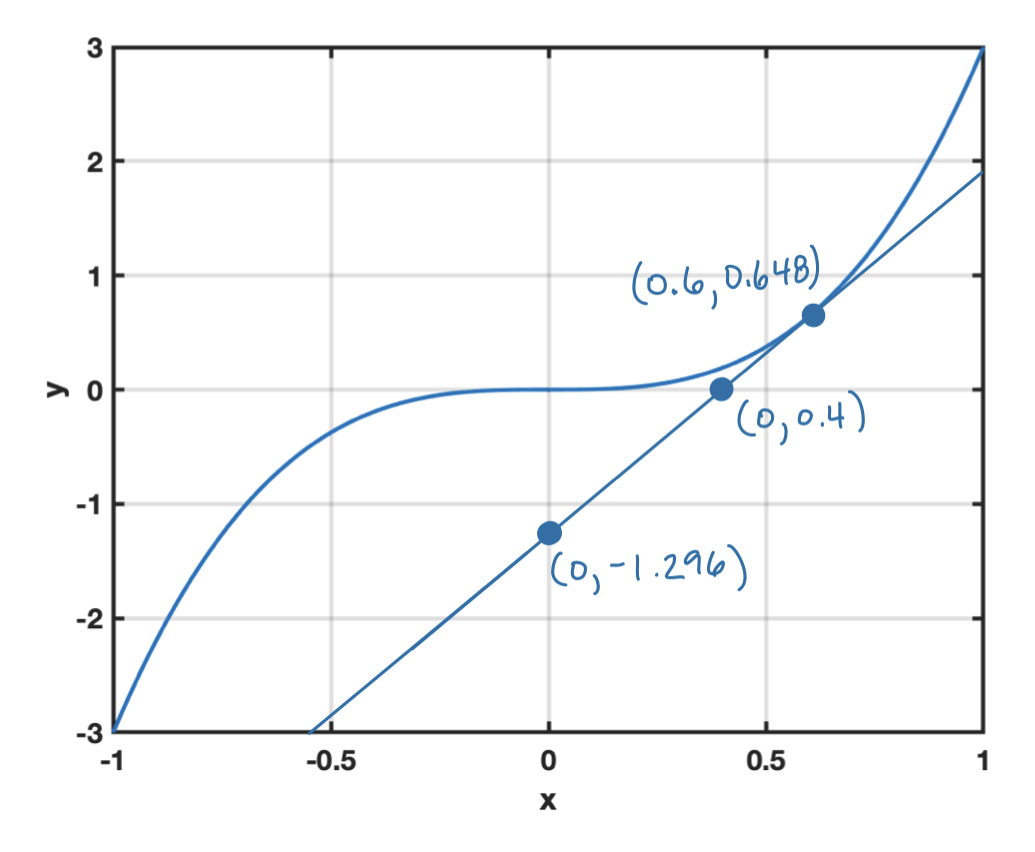
\includegraphics[width=0.55\textwidth]{PS1-Fig2.png}
            % \caption{}
            % \label{fig:Title}
        \end{figure}
        \item On the diagram above, sketch the linear approximation. Hand this in with your completed assignment.
    \end{enumerate}
    \item (+10 points) Consider the linear op-amp circuit shown below.
    \begin{figure}[h!]
        \centering
        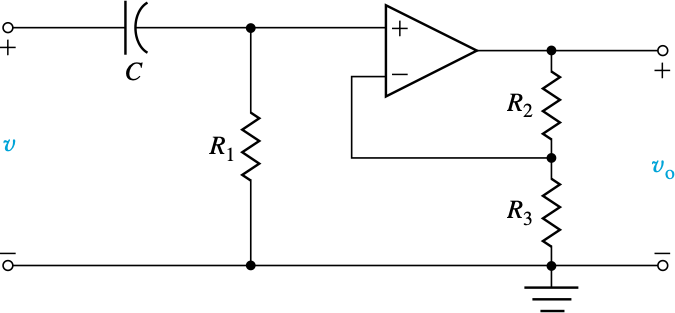
\includegraphics[width=0.5\textwidth]{PS1-Fig3.png}
        % \caption{}
        % \label{fig:Title}
    \end{figure}
    \begin{enumerate}
        \item Assuming all initial conditions are zero, find the transfer function \( G(s)=V_0(s) / V(s) \). \textit{For full credit, write the transfer function in standard polynomial form (i.e., no fractions in \(s\) in the numerator or denominator)}
        \begin{align*}
            C\frac{dv}{dt}+v(t)&=v_0(t)\left[ \frac{R_2}{R_2+R_3}\right]\\[0.5em]
            CsV(s)+\frac{V(s)}{R_1}&=V_0(s)\left[ \frac{R_2}{R_2+R_3}\right]\\[0.5em]
            V(s)\left[Cs+\frac{1}{R_1}\right]&=V_0(s)\left[ \frac{R_2}{R_2+R_3}\right]\\[0.5em]
            G(s)=\frac{V_0(s)}{V(s)}&=\frac{R_1Cs\left(R_2+R_3\right)}{R_2R_1Cs+1}
        \end{align*}\newpage
        Now assume that \(C=1,R_1= 1,R_2=2,R_3= 1\) (unit-less quantities).
        \item What is the system response \(v_0(t)\) to a step \(v(t)=\bm{1}(t)\)?
        \begin{align*}
            \frac{V_0(s)}{V(s)}&=\frac{\cancelto{3s}{R_1Cs\left(R_2+R_3\right)}}{\cancelto{2s+1}{R_2R_1Cs+1}}\\[0.5em]
            V_0(s)&=\frac{V_0(s)}{V(s)}\cdot \frac{1}{s}\\[0.5em]
            &=\frac{3\cancel{s}}{2s+1}\cdot \frac{1}{\cancel{s}}\\[0.5em]
            &=\frac{3}{2s+1}
        \end{align*}
    \end{enumerate}
\item (+10 points) Consider the spring mass damper system shown on the next page with \(m_1=m_2=1\) kg, \(k_1=k_2=1\) N/m. Note that you can neglect gravity by considering deviations from the system at rest.
    \begin{enumerate}
        \item Draw a free-body diagram for each mass. Write the equations of motion in terms of \(x(t)\) and \(y(t)\) and their derivatives. Presume zero initial conditions.
        \begin{center}
            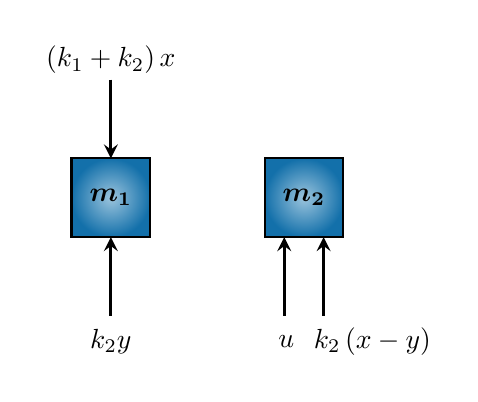
\begin{tikzpicture}
                \matrix[column sep=1cm]{
                    \filldraw[inner color=InnerBlue,outer color=OuterBlue, thick] (0,0)rectangle (1,1);
                    \draw[->, very thick](0.5,-1)--(0.5,0);
                    \draw[->, very thick](0.5,2)--(0.5,1);
                    \node at (0.5,0.5) {$\bm{m_1}$};
                    \node at (0.5,-1.33) {$k_{2}y$};
                    \node at (0.5,2.25) {$\left(k_1+k_2\right)x$};
                &
                    \filldraw[inner color=InnerBlue,outer color=OuterBlue, thick] (0,0)rectangle (1,1);
                    \draw[->, very thick](0.75,-1)--(0.75,0);
                    \draw[->, very thick](0.25,-1)--(0.25,0);
                    \node at (0.5,0.5) {$\bm{m_2}$};
                    \node at (0.5,-1.33)[left] {$u$};
                    \node at (0.5,-1.33)[right] {$k_2\left(x-y\right)$};\\
                };
            \end{tikzpicture}
        \end{center}
        \begin{align*}
            m_1\ddot{x}&=-(k_1+k_2)x+k_2y\\
            m_2\ddot{y}&=u+k_2(x-y)
        \end{align*}
        \item What is the transfer function with input \(U(s)\) and output \(X(s)\)?\\[1em]
        Plugging in our given constants, we obtain:
        \begin{align*}
            \ddot{x}=-2x+y\qquad\rightarrow\qquad s^2X(s)&=-2X(s)+Y(s)\\
            \ddot{y}=x+y+u\qquad\rightarrow\qquad s^2Y(s)&=X(s)-Y(s)+U(s)\\
            s^2Y(s)+Y(s)&=X(s)+U(s)\\
            Y(s)\left[s^2+1\right]&=X(s)+U(s)\\
            Y(s)&=\frac{X(s)+U(s)}{s^2+1}
        \end{align*}
        Next, plugging \(Y(s)\) into our function for \(X(s)\).
        \begin{align*}
            s^2X(s)&=-2X(s)+Y(s)\\
            s^2X(s)&=-2X(s)+\frac{X(s)+U(s)}{s^2+1}\\
            \left[s^2X(s)+-2X(s)\right]\cdot\left[s^2+1\right]&=X(s)+U(s)\\
            s^4X(s)+s^2X(s)+3X(s)&=U(s)\\
            \frac{X(s)}{U(s)}&=\frac{1}{s^4+s^2+3}
        \end{align*}

    \end{enumerate}
\item (+10 points) For this exercise, you will hand in a history of Matlab command-line inputs and outputs (so do not silence the output with ‘\texttt{;}’).  Use \texttt{diary} or \texttt{publish} to record your session. To use the commands below, note that it is almost always helpful to refer to Matlab’s \texttt{help} command or to the online documentation.\par
Consider the following transfer function:
    \begin{align}
        G(s)=\frac{4}{(s+1)(s+4)}
    \end{align}
    \begin{enumerate}
        \item Find the coefficients of the polynomial in the denominator using the \texttt{conv} command. Your answer should be of the form \text{[1 x y]}, with \(x\) and \(y\) representing numerical values.\\[1em]
        (For parts (a) through (c), please see attached Matlab code below.)
        \item Find the roots of the denominator using the \texttt{roots} command on your answer to the previous question.
        \item Construct the transfer function \(G(s)\) via the \texttt{tf} command.
        \item Calculate the step response of \(G(s)\) via the \texttt{step} command. Compare your step response to the  one  below,  which  is  computed  for  the  system \(G_2(s)=\frac{4}{s^2+s+4}\). What are the significant similarities and differences between the two responses and transfer functions? Do the step responses appear to have any oscillatory component? (You do not need to hand in the plot of the step response, but may do so if it aids in your discussion.)\\[1em]
        The two transfer functions are very similar in their end pattern; however, the second function, \(G_2(s)\), has an oscillatory component as shown in orange on the attached Matlab graph. The original transfer function, \(G(s)\), lacks this oscillation due to the slight change in the second term of its denominator.
    \end{enumerate}
\end{enumerate}
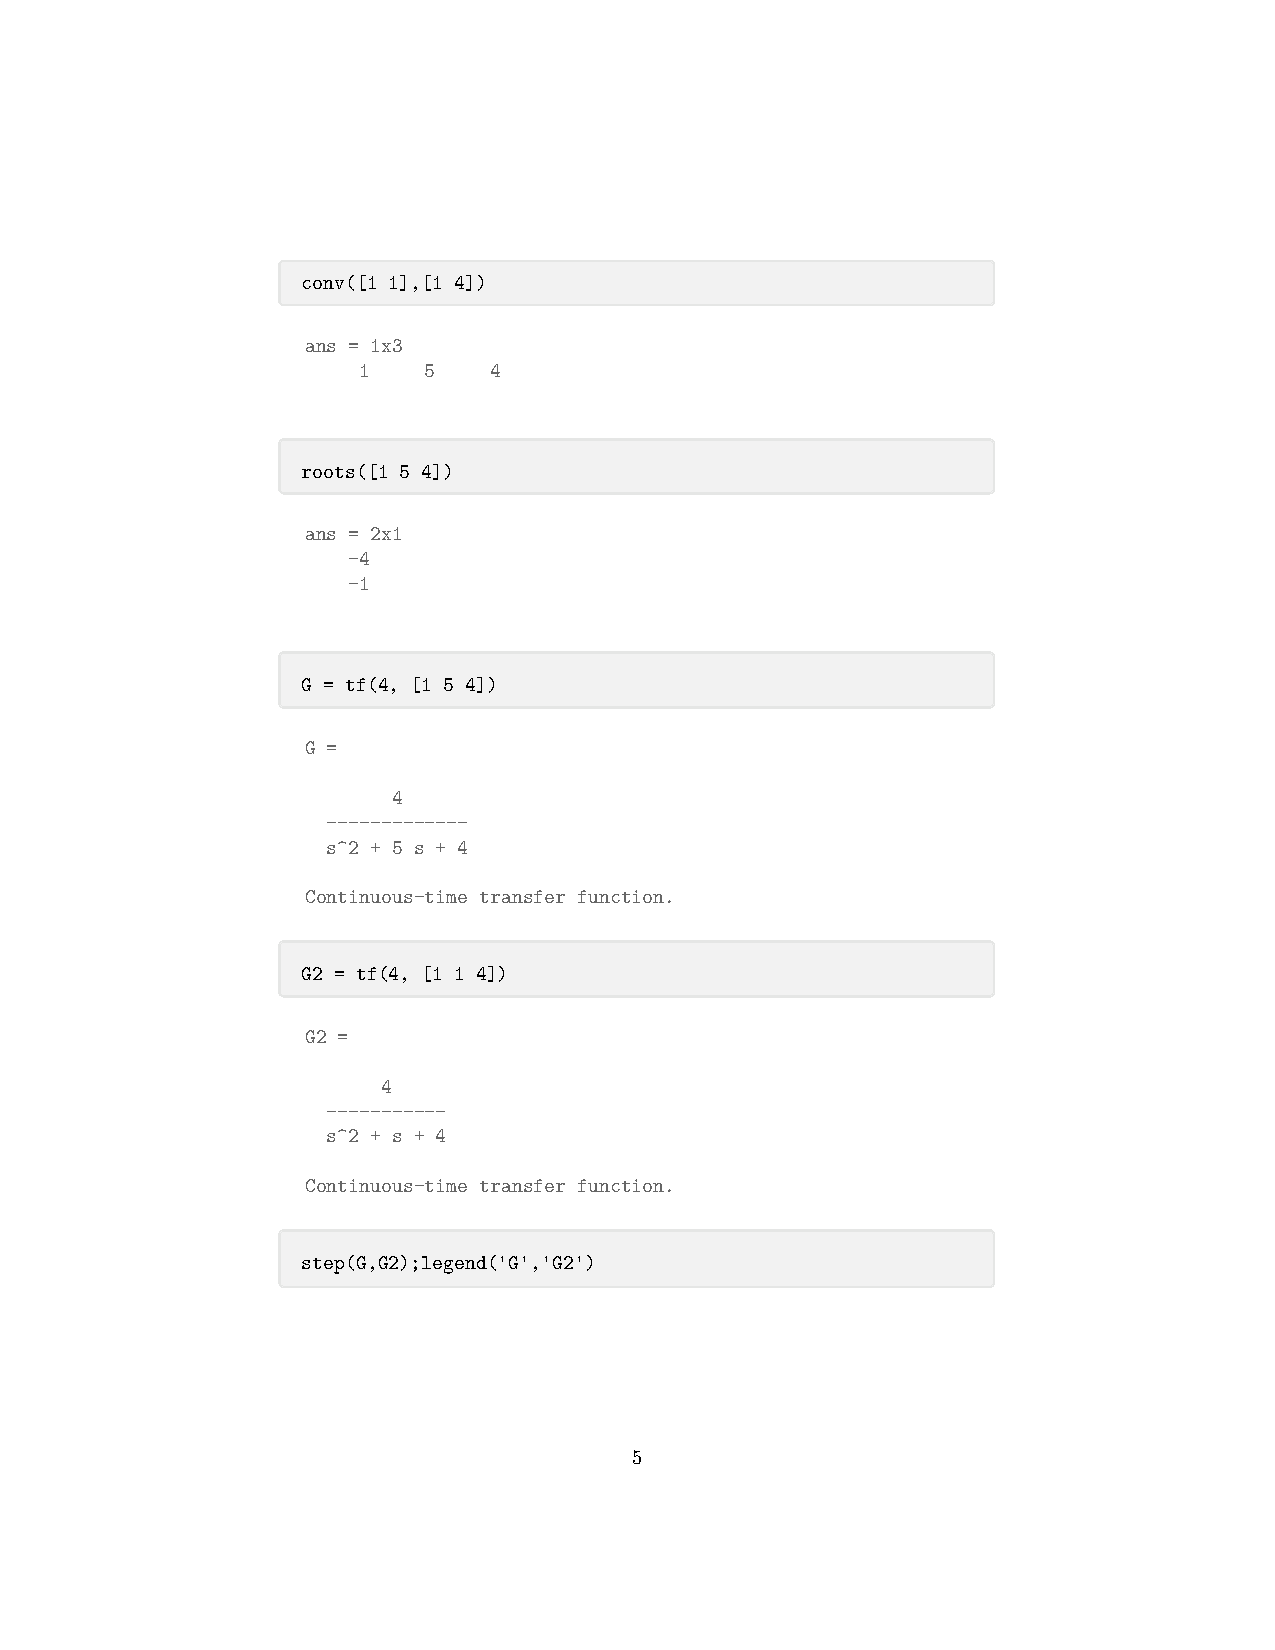
\includepdf[pages=-]{PS1-Matlab.pdf}

\end{document}